%Move from macro to micro, citing from oldest references to the most recent

%What it is: 
%–Overview of previous work in the field 
%– What’s the big picture?
%–Explanation of how your work addresses the gap in the field
%–Enough technical details for the reader to understand your project
%–Explanation of importance/impact of your work 

%What you need to show: 
%–You understand what’s going on in your field, and how your work fits into that. 
%–You have the authority to say your research is important/novel. 

%Can be helpful to... 
%–Restate your hypothesis 
%–Briefly mention an experimental overview (just enough to lead the reader into your Project Plan)


%Disadvantage to Bayesian Fit and MCMC: These include the subjectivity induced by choice of prior as well high computational costs
In this section, we will talk about a brief background to Neural Networks and the types of neural networks, leading to the architecture of a Recurrent Neural Network, it's types and it's uses. We will then address some related work in the field of Transit detection, focusing majorly on the vetting. 
\subsection{Neural Networks}
Machine Learning is a type of computer algorithm that is used to predict certain outputs based on the input data. The heuristics of what to learn from the data are automatically identified in the data by this machine learning model in a process called \emph{"Training"}. A supervised machine learning model typically requires a set of inputs and their corresponding actual outputs or labels. The task of the model in the training process is to minimize the difference between the predicted mathematically calculated output it gives based on the certain set of inputs and the actual output, as calculated by a cost function.\\

Deep Learning is a sub-class of Machine Learning which uses mathematical sub-units called neurons. Each of these neurons are arranged in layer like format, where every neuron from one layer is connected to every other neuron in the next layer. The connections between these neurons are called weights, which are multiplicative factors, and each neuron has a bias attached to it, leading to their configuration as
\begin{center}
$a_i = f(W_i * x\textsubscript{i-1} + b_i)$
\end{center}

where $a_i$ is the output of neuron layer \emph{i} when $x\textsubscript{i-1}$ is the input from the previous (\emph{i-1}) layer neurons and the function $f()$ is an activation function which induces non-linearity. Figure below shows a Fully Connected Neural Network or a Multi-layered perceptron. 

%Figure
\begin{figure}[H]
    \centering
    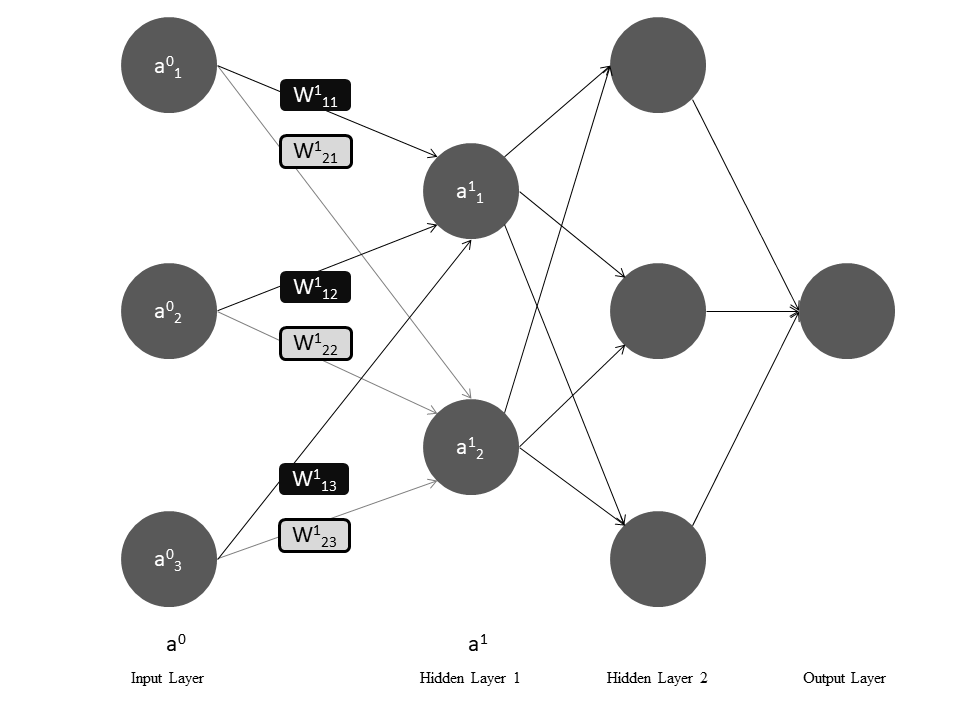
\includegraphics[scale=0.4]{Images/ANN.png}
    \caption{A Fully Connected Neural Network with 2 Hidden Layers. Connections weights are shown between Input layer and Hidden layer 1}
    \label{fig:ANN}
\end{figure}

The \textbf{backpropagation algorithm} changes these weights and biases of the neurons in order to minimize the cost function. Cross Entropy loss is calculated as the cost function for binary classification problems. In order to minimize the cost, we take gradient of the cost (first order derivative) with respect to the parameters of the model and equate it to 0. This indicates the iterative updation of parameters till a minima for the cost is reached, which indicates the optimal model performance.  \\

\textbf{Convolutional Neural Networks} are a class of neural networks which use convolution (or discrete cross-correlation) operation on the input with a kernel/filter at the convolution layer, which is fed to the pooling layer to reduce the dimensionality of the resulting \emph{feature map} by aggregating regions in the neighbouring proximity using mean or maximum values, the output of which is finally fed to a fully connected layer for the prediction of the output. The output of the convolutional layer, or the feature map is given by \\
\begin{center}
    $a_i^{(l)} = f(\sum_{k=1}^K w_i^{(k,l)} * a_{i-1}^{(k)} + b_i^{(l)})$
\end{center}
where the $K$ vectors of length $n_{i-1}$ are input to the $i^{th}$ layer (k=1,2, ..., K) given by $a_{i-1}^{(k)}$, L is the output number of vectors (l=1,2, ...,L) given by $a_i^{(l)}$, $f()$ is the activation function, $*$ is the convolution function, $w_i^{(k,l)}$ is the weight array acting as a filter or kernel and $b_i^{(l)}$ are the bias vector.


\subsection{Recurrent Neural Networks}
Recurrent neural networks are yet another class of NNs which feed the network output back as an input to the network. This allows them to retain information, identify patterns and establish temporal connections, which is suitable for time-series applications.
\begin{figure}[h]
    \centering
    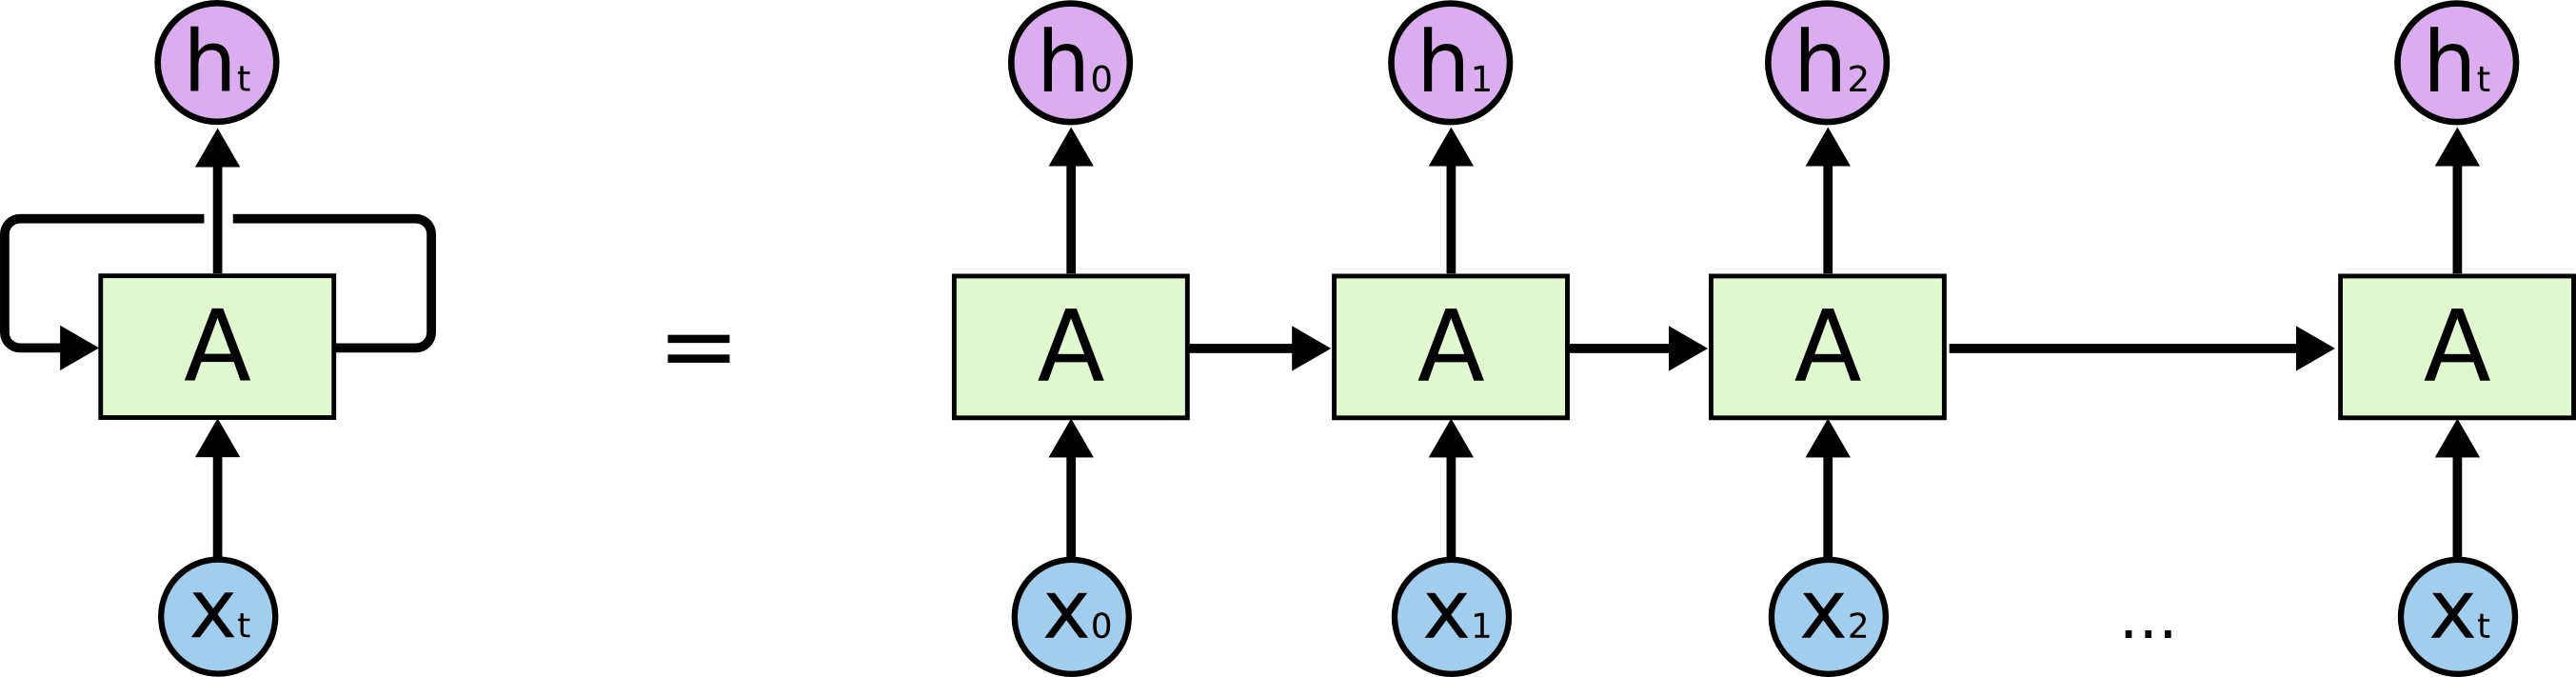
\includegraphics[scale=0.3]{Images/RNNs_1.png}
    \caption{A Recurrent Neural Network. The looped layers are shown unrolled here. \emph{Source}: \href{https://colah.github.io/posts/2015-08-Understanding-LSTMs/}{\textit{Understanding LSTM Networks, Colah 2015}}}
    \label{fig:RNN}
\end{figure}
Long Short Term Memory Networks are a type of gated RNNs that can learn long term dependencies between the data points by removing or adding certain information through the sigmoid gates, controlling this flow of information. There is a Cell-state which flows through the LSTM cells. The information which we need to remove is decided by the first sigmoid gate. The second sigmoid gate in conjecture with $tanh$ of the previous state's output decides what we keep in the cell state. This cell state then factors in with a $tanh$ to the current state's output.
\begin{figure}[h]
    \centering
    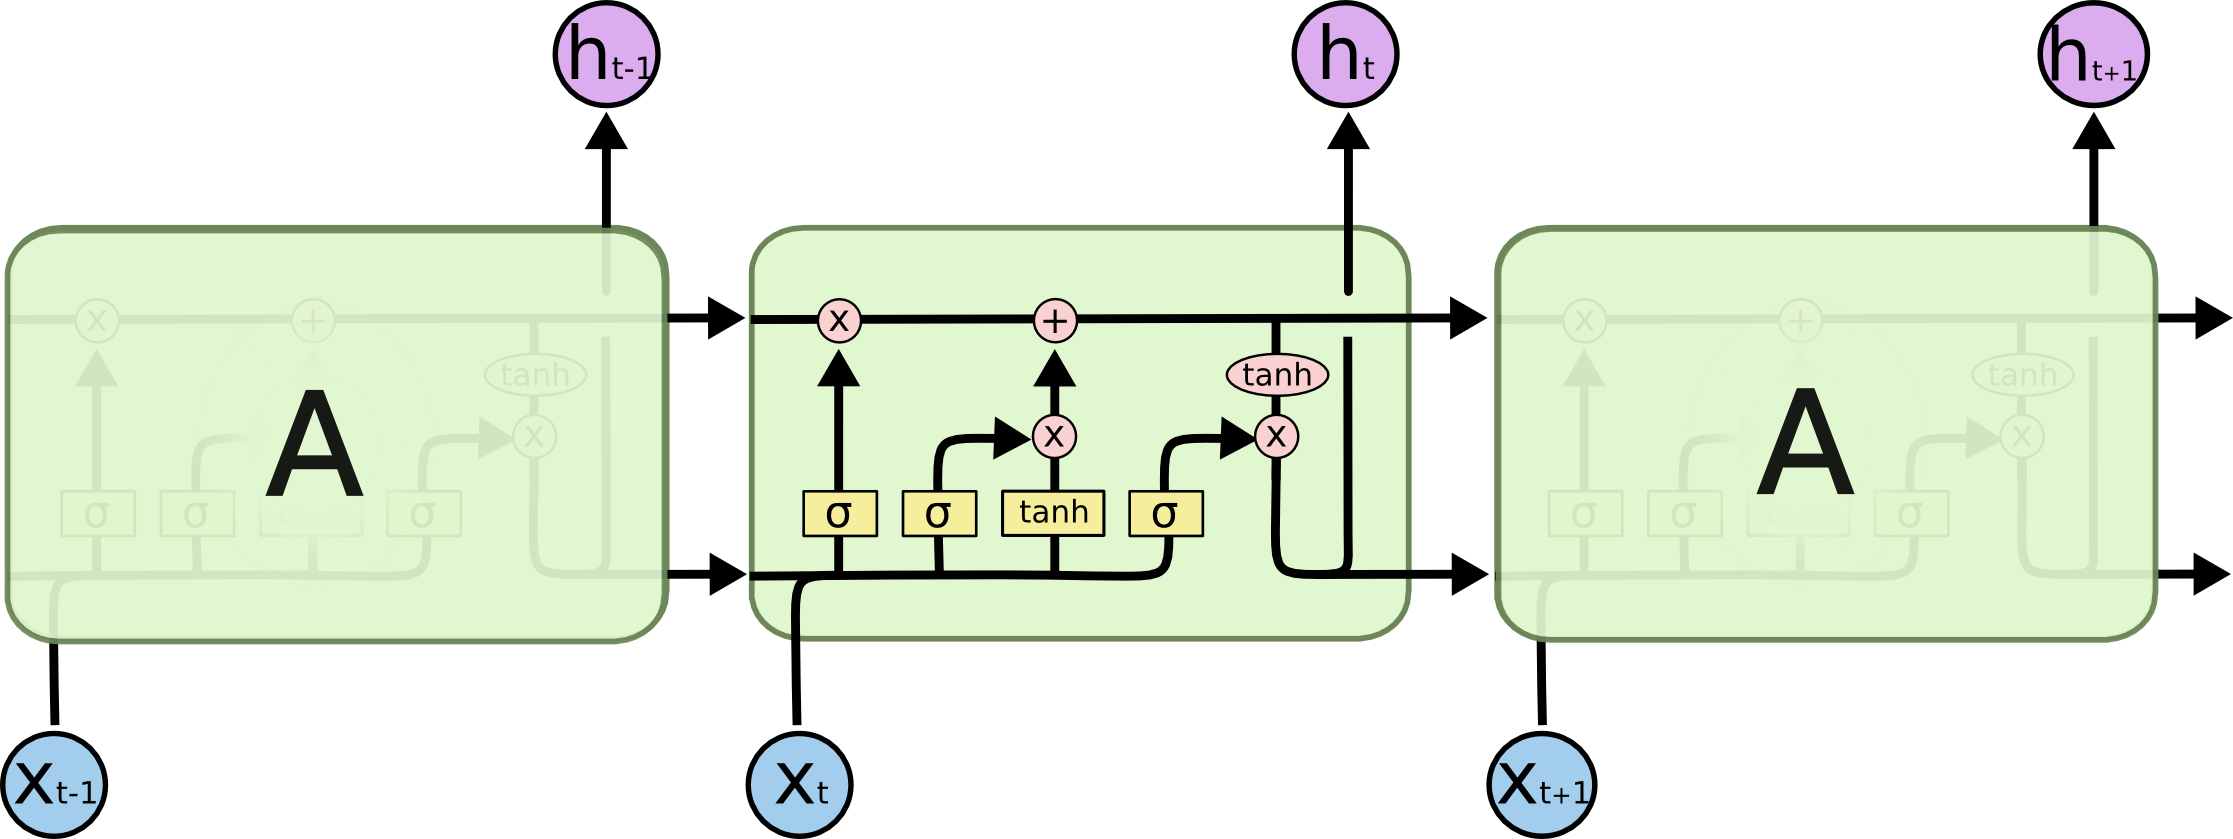
\includegraphics[scale=0.35]{Images/LSTM.png}
    \caption{Simplified architecture of Long Short Term Memory Network. \emph{Source}: \href{https://colah.github.io/posts/2015-08-Understanding-LSTMs/}{\textit{Understanding LSTM Networks, Colah 2015}}}
    \label{fig:LSTM}
\end{figure}
\subsection{Transit Classification}
Transit detection for exoplanets is a field involving space-based high precision photometry. A dip in the stellar flux/brightness indicates a transiting phenomena occuring, or in simpler terms, something is passing between the field of vision from the telescope and the star. We record the stellar lights over a time span and the resulting flux time series is calles a \emph{Light Curve}
\begin{figure}[h]
    \centering
    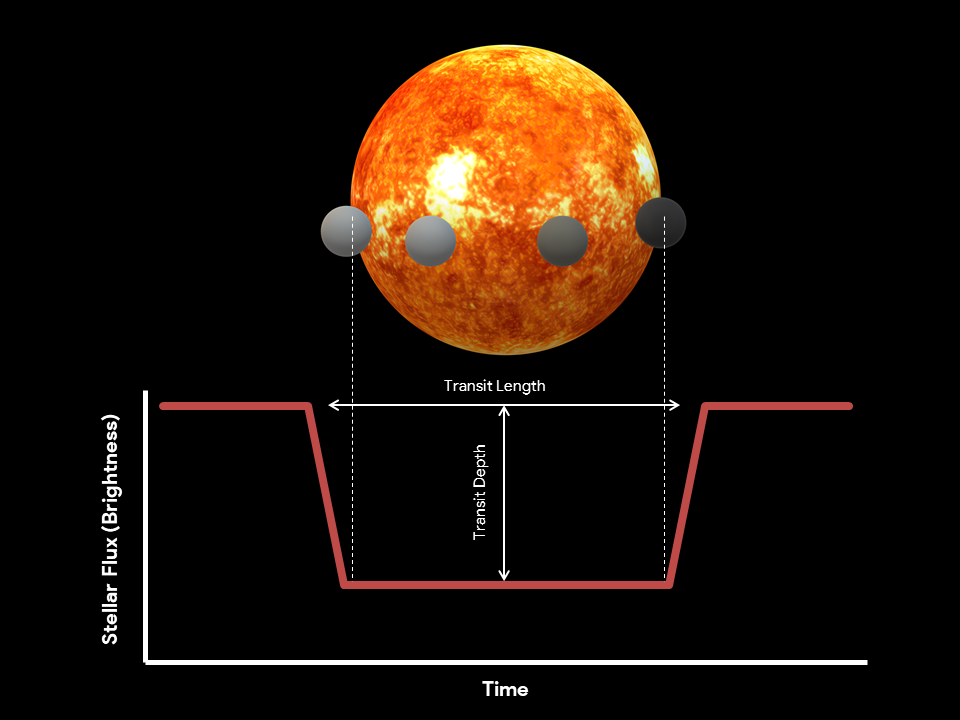
\includegraphics[scale=0.4]{Images/Transit.png}
    \caption{Stellar light curve plotted against a planet transiting it's host star}
    \label{fig:Transit}
\end{figure}

